\section{Introducción}

El objetivo de la metodología descripta en este capítulo consiste en revisar el compilador y lenguaje de Solidity, analizar su diseño general y arquitectura, y reportar potenciales vulnerabilidades de seguridad que puedan llegar a comprometer el código compilado. En este capítulo se describe el trabajo realizado presentando ejemplos de observaciones en áreas específicas del código que presentan problemas concretos, así como también observaciones generales que atraviesan el proyecto entero, que puede mejorar su calidad como un todo.\\

Se puede interpretar a la metodología como una auditoría abarcativa, no sólo de seguridad, sino en todos los aspectos que permitan encontrar problemas. No es menor resaltar que cualquier problema en este contexto puede ser considerado un potencial impacto de seguridad.\\

El método propuesto no tiene intención de destacarse por utilizar características novedosas a nivel tecnológico o introducir nuevos procesos. De hecho todo lo que se realizará en esta sección, no es más que, en distintas medidas, una conjunción de los dos capítulos anteriores, y es por eso que parece importante hacer énfasis en este tipo de propuestas, ya que están al alcance del estado del arte.\\

La razón de centrar el foco de investigación en un proyecto open source, que posee instrucciones sobre cómo construirlo, y una documentación extensa, es para presentar una situación favorable y menos limitante para realizar una auditoría. No obstante, poseer esta situación lo hace más complejo y desafiante, ya que se puede analizar desde todas las perspectivas posibles.\\

Su código está disponible online, y se ha decidido congelar el repositorio en la última versión estable a la hora de realizar esta investigación.


\section{Alcance de la auditoría}

El código auditado puede encontrarse en su repositorio público de GitHub ethereum/solidity\cite{SolidityGitHub}, y la versión utilizada para el análisis se encuentra en el \textit{tag} v0.4.24\cite{SolidityGitHub0424}, commit: \texttt{e67f0147998a9e3835ed3ce8bf6a0a0c634216c5}.\\

La auditoría contendrá un profundo análisis, diseño e implementación de la herramienta, apuntando a asesorar su calidad e investigar problemas potenciales que pueden surgir mediante su utilización.\\

Estas actividades incluyen revisar las etapas de \textit{parsing}, análisis, optimización, código de generación. La auditoría cubrirá el código ensamblador generado para la \textit{EVM}, \textit{ABIs} (Application Binary Interface), y Solidity con código intermedio \textit{Yul} de manera \textit{inline}.\\

No se cubrirá la generación de código \textit{eWASM} (Ethereum Flavored WebAssembly), las características relacionadas al lenguaje \textit{LLL} (lenguaje de bajo nivel para la \textit{EVM} con una sintaxis de expresiones-s ), las características experimentales, y las herramientas de verificación formal incluídas en el proyecto.\\

El proyecto no parece integrar la seguridad como componente activo en su ciclo de desarrollo. Incluye un componente para aplicar técnicas de \textit{fuzzing} y una suite de testeo. Estos no serán analizados con detenimiento pero de todos modos se verá cuál es su real interacción con el compilador.

\section{Metodología }
\label{chap:metodo:metodologia}
Para estos casos, siempre es mejor realizar una revisión manual de código, y como tal se debe comenzar con un modelado de amenazas o al menos entrevistas a los desarrolladores para tener un entendimiento de la arquitectura de la aplicación, su superficie de ataque, así como también las técnicas de implementación.\\

Es por eso que durante toda la auditoría se mantuvo siempre al menos un canal de comunicación abierto con el equipo encargado del proyecto. Se utilizaron servicios de mensajería\cite{GitterLink} para mantener un diálogo específicamente para detalles asíncronos sobre dudas puntuales, frecuentemente relacionadas a la información presentada en el repositorio de \textit{GitHub}.\\

\textit{GitHub} como herramienta fue utilizada en el proyecto como medio de intercambio de información de una manera más acoplada al proyecto, teniendo la posibilidad de continuar involucrando a la comunidad activa.\\

Finalmente para partes del código difíciles de comprender, se realizaron \textit{walkthroughs} (guías destinadas a mejorar el entendimiento del proyecto) mediante videollamadas en una herramienta de videoconferencia\cite{MeetLink}.\\ 

Se utilizó un conjunto de las estrategias de auditoría de código con propósitos bien definidos. Por ejemplo, la \textit{generalización de diseño} aplicada a analizar la arquitectura del compilador; \textit{puntos candidatos} para posibles problemas en las etapas de parsing y optimización; y \textit{compresión de código} basados en hallazgos mediante técnicas de \textit{black box} o \textit{testing} manual. Para una representación gráfica aproximada ver Figura \ref{fig:metodologia}.\\

\begin{figure}[ht]
    \centering
    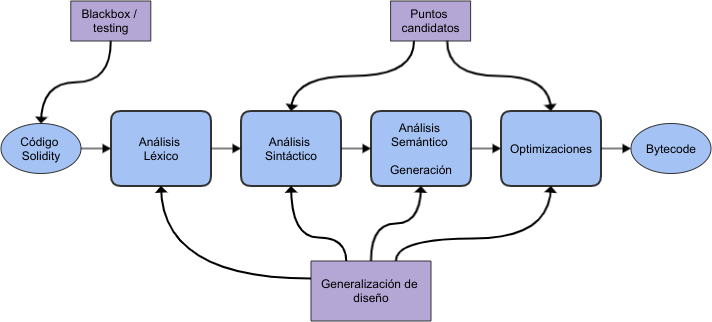
\includegraphics[scale=0.5]{images/methodology.png}
    \caption{Estrategias aplicadas, visualización.}
    \label{fig:metodologia}
\end{figure}

A grandes rasgos, se pretendió:
\begin{itemize}
    \item Cubrir un análisis general del proyecto en todos los aspectos del mismo, desde cómo está conformado el equipo que lo mantiene hasta las tecnologías que se utilizan.
    \item Realizar revisión de código en los puntos candidatos y en los lugares en donde se han  producido fallos en las pruebas de \textit{black box}.
    \item Auditar las distintas etapas del compilador a nivel general, buscando que la arquitectura del compilador contemple las etapas estándar.
    \item Revisar el diseño del lenguaje y su instrumentación para verificar que la instrumentación sea consistente con la especificación del diseño del lenguaje.
    \item Revisar la configuración de testeo para detectar posibles fallos en los códigos de testeo del propio proyecto.
    \item Aplicar técnicas de black box para identificar el lugar del fallo y el lugar y la magnitud del impacto del mismo.
    \item Analizar la salud del proyecto para hallar posibles defectos como compatibilidad hacia atrás, aspectos no contemplados, información inconsistente y sin tratamiento en los repositorios, entre otros.
    \item Revisión de problemas previamente reportados para asegurar el tratamiento y seguimiento de temas ya identificados.
    \item Análisis de la documentación para verificar la consistencia entre la documentación y los aspectos de sintaxis, semántica y pragmática del compilador.
\end{itemize}
\bigskip

Finalizar una auditoría no consta únicamente de entregar lo hallado de manera descriptiva. Se cumple un rol muy importante a la hora de presentar los resultados, ya que sin alternativas, soluciones o sin mantener un contacto para ayudar a remediar los problemas reportados estaría faltando una parte muy importante del trabajo. Frente a los hallazgos se proponen también recomendaciones a aplicar para mejorar la calidad del proyecto.

\section{Herramientas par el análisis}

El método principal de análisis comienza observando y comprendiendo el código (escrito en el lenguaje C ++, versión 11) del compilador en profundidad. Sin embargo, también se utiliza una serie de herramientas automatizadas que ayudan el estudio en varios aspectos complementarios. Estos se estructuran en 3 categorías principales: (1) \textit{visualización de código}, (2) \textit{análisis estático} y (3) \textit{prueba / fuzzing}. Estas categorías se aplican tanto para el código \textit{C++} del compilador como para la salida \textit{EVM} que genera.

\subsubsection{Herramientas C++ (Código del compilador)}

Debido a que \textit{C++} es un lenguaje establecido que contiene cierta madurez, existe una gran cantidad de herramientas disponibles. Las herramientas de visualización nos ayudan a comprender el código del compilador, así como a navegarlo. Las herramientas de análisis estático nos ayudan a detectar las dificultades semánticas comunes dentro de él, y las herramientas de \textit{fuzzing} estresan al compilador con un gran conjunto de pruebas generadas automáticamente.\\

\textbf{Visualización de código (C++):}\\

\underline{\textit{SourceTrail}}\cite{SourceTrailLink}
Un explorador de código para \textit{C++} y \textit{Java}. Extremadamente útil para la rápida navegación visual de una gran base de código.\\

\underline{\textit{Visual Paradigm}}\cite{VisualParadigmLink}
Una herramienta para generación de gráficos \textit{UML}. Permite generar distintos diagramas, como el de clases, basándose en el código de un proyecto.\\

\underline{\textit{Ctags}}\cite{CtagsLink}
Indexador de código. Comúnmente utilizado junto con el IDE para facilitar la navegación del proyecto.\\

\underline{\textit{Cscope}}\cite{CscopeLink}
Navegador de código de fuente. Es similar a Ctags pero permite ir un poco ``más allá", y funciona mejor en proyectos grandes donde su código no es conocido.\\

\underline{\textit{Clang-tidy}}\cite{ClangTidyLink}
Linter basado en Clang para C++ apuntado a diagnosticar y señalar típicos errores de programación. Incluye chequeos para las librerías de boost también.\\

\underline{\textit{CppCheck}}\cite{CppCheckLink}
Herramienta de análisis estático para C++ apuntado a detectar errores reales (mínimos falsos positivos).\\

\underline{\textit{CppDepend}}\cite{CppDependLink}
Potente análisis estático destinado a mejorar la calidad del código.\\

\underline{\textit{Flawfinder}}\cite{FlawfinderLink}
Herramienta para detectar posibles problemas de seguridad en código C++.\\

\underline{\textit{CppLint}}\cite{CppLintLink}
Es una herramienta de línea de comandos para verificar archivos C / C ++ en busca de problemas de estilo siguiendo la guía de estilo C++ de Google.\\

\underline{\textit{Scan-build}}\cite{ScanBuildLink}
Es una utilidad de línea de comando que permite a un usuario ejecutar un analizador estático sobre su base de código como parte de la realizar una compilación regular.\\

\underline{\textit{Lizard}}\cite{LizardLink}
Lizard es un analizador de complejidad ciclomática extensible para muchos lenguajes de programación, incluido C/C++ (no requiere todos los archivos de encabezado ni las importaciones de Java). También realiza detección de copy \& paste (detección de clon de código / detección de duplicado de código) y muchas otras formas de análisis de código estático.\\

\textbf{Prueba / fuzzing (C++):}\\

\underline{\textit{Grammarinator}}\cite{GrammarinatorLink}
Genera pruebas aleatorias de acuerdo con una definición de gramática ANTLR. La gramática Solidity.g4\cite{SolidityG4} creada por Federico Bond permite un acercamiento menos laborioso para integrar la gramática oficial.\\

\underline{\textit{American Fuzzy Lop}}\cite{AFLLink}
AFL es un fuzzer orientado a la seguridad que emplea un nuevo tipo de instrumentación en tiempo de compilación y algoritmos genéticos para descubrir automáticamente casos de prueba limpios e interesantes que desencadenan nuevos estados internos en el binario objetivo. Esto mejora sustancialmente la cobertura funcional para el código fuzzeado.\\

\underline{\textit{LibFuzzer}}\cite{LibFuzzerLink}
Es un motor evolutivo de fuzzing, in-process, guiado por la cobertura del proyecto. Se enlaza con la biblioteca o el proyecto bajo testeo, y se le alimenta entradas fuzzeadas mediante un punto de entrada; el fuzzer luego localiza qué áreas del código son alcanzadas, y genera mutaciones a partir de los datos de entrada para maximizar la covertura del código.\\
La información de cobertura del código para libFuzzer es proporcionada por la instrumentación SanitizerCoverage de LLVM.\\

\underline{\textit{Instrumentaciones de compilación de Clang}}\cite{ClangInstrumentationLink}
Flags de compilación para instrumentar en compilación al binario.
AddressSanitizer\cite{AddressSanitizerLink} (detector de error de memoria rápida), MemorySanitizer\cite{MemorySanitizerLink} (detector de lecturas de variables no inicializadas), Fuzzer (alternativa para utilizar libFuzzer), SanitizerCoverage\cite{SanitizerCoverageLink} (cobertura de código).\\

\underline{\textit{Debugging: gdb/lldb\cite{gdbLink}\cite{lldbLink}}}
Herramientas de debugging para realizar análisis en ejecución. Se pueden utilizar como línea de comandos, o integrados al IDE.\\

\underline{\textit{Dhex}}\cite{DhexLink}
Editor hexadecimal por línea de comandos.\\

\underline{\textit{Honggfuzz}}\cite{HonggfuzzLink}
Fuzzer orientado a la seguridad con potentes opciones de análisis. Admite fuzzing evolutivo basado en retroalimentación basado en la cobertura de código (basado en software y hardware).

\subsubsection{Herramientas EVM (Código generado por el compilador)}

El ecosistema \textit{Ethereum} ya está produciendo una serie de herramientas que son potencialmente útiles para este análisis. Las herramientas de visualización ayudan a comprender el resultado del compilador, que es bastante bajo y difícil de leer de forma natural. Dicha visualización es particularmente importante para evaluar las optimizaciones del código de operación \textit{EVM}. El análisis estático ayuda a identificar problemas de flujo de control que pueden impactar la \textit{EVM}, y las herramientas de fuzzing nos permiten probar bytecode fuera de la interfaz \textit{ABI} ampliamente utilizada actualmente cubierta en muchos frameworks.\\

\textbf{Visualización de código (EVM):}\\

\underline{\textit{Solplay}}\cite{SolplayLink}
Visualizador de Solidity a varias salidas del compilador, incluyendo procesamiento post-bytecode por otras herramientas. Creada por Zeppelin particularmente para esta auditoría, intencionada para acelerar el uso de otras herramientas de visualización.\\

\underline{\textit{Solmap}}\cite{SolmapLink}
Bytecode visualizado en tiempo real, con la habilidad de seleccionar conjuntos de instrucciones y ver el código en Solidity asociado a ellos. Utiliza la información de mapeo de código de Solidity. También construida por Zeppelin para esta auditoría.\\

\underline{\textit{Remix}}\cite{RemixLink}
Solidity IDE web. Útil para debuggear salidas del compilador. \\

\underline{\textit{Evmdis}}\cite{EvmdisLink}
Disassembler para la EVM que agrupa opcodes en expresiones más legibles. Útil para visualizaciones pero no es 100\% preciso.\\

\underline{\textit{go-ethereum/evm}}\cite{goEthereumLink}
Utilidad para desarrolladores de la EVM. Excellente para debuggear la ejecución de la EVM a un bajo nivel.\\

\underline{\textit{Evm-tools}}\cite{evmToolsLink}
Herramientas para la ejecución y el desensamblado de la EVM. Tools for EVM execution. Desactualizado, pero útil principalmente con fines educativos. No es lo suficientemente confiable.\\

\textbf{Análisis estático (EVM):}\\
Fuera del alcance de la investigación.\\

\textbf{Prueba / fuzzing (EVM):}\\

\underline{\textit{Web3}}\cite{Web3Link}
Ethereum Javascript API.\\

\underline{\textit{Geth}}\cite{GethLink}
Implementación en Go de un nodo de ethereum, utilizado para simular transacciones y correr testeos.\\

\underline{\textit{Cpp-ethereum}}\cite{cppEthereumLink}
Implementación de nodo en Ethereum en C++.\\

\section{Formato de los resultados}
La manera más oportuna y organizada de presentar los resultados, dada la cantidad y la complejidad que poseen, se concluyó que debería ser compuesta de un título descriptivo, un breve desarrollo de la situación en la que se da, un ejemplo o forma de replicación, recomendaciones para remediar o mejorar esa situación, y para finalizar un breve comentario con el estado actual de dicha cuestión en el proyecto.\\

El estado actual no es más que una sección comentando la respuesta por parte de los líderes del proyecto, y el estado en el que se encuentra a la hora de escribir este trabajo de investigación, que difiere notablemente de la fecha de los hallazgos. Se incluirán links a \textit{issues} (especie de tickets para reportar problemas, sugerencias, y más) y \textit{pull requests} (solicitud de incorporación cambios) de \textit{GitHub} en los casos en los que existan referencias directas con el proyecto.
